
\section{Introduction}

\begin{frame}{Motivation}
  \begin{figure}
    \centering
    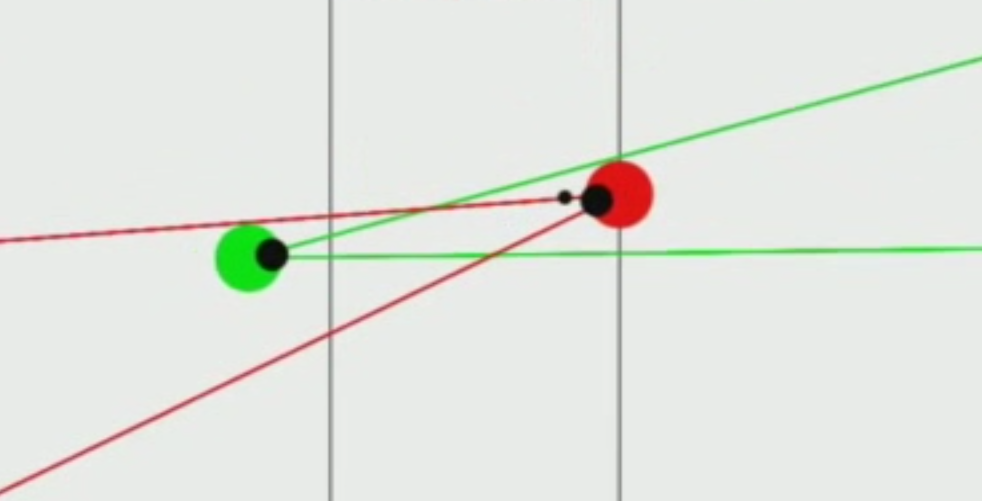
\includegraphics[width=250px]{elias/images/sniper.png}
    \caption{\url{youtube.com/watch?v=u2t77mQmJiY}}
    %by Ding Nicolas
  \end{figure}
\end{frame}

\begin{frame}{Motivation}
  \begin{figure}
    \centering
    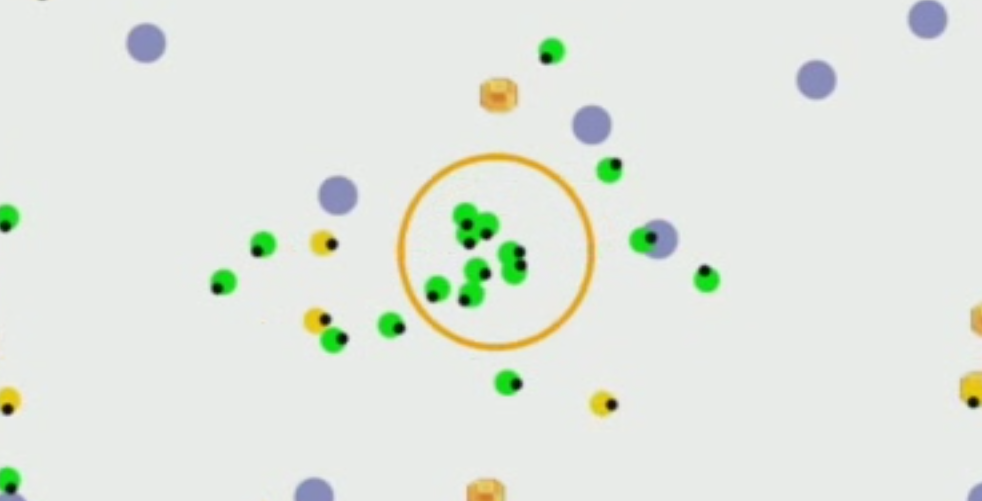
\includegraphics[width=250px]{elias/images/swarm.png}
    \caption{\url{youtube.com/watch?v=Iv_Fy6Urik4}}
    %by Ding Nicolas
  \end{figure}
\end{frame}

\begin{frame}{Motivation}
  \begin{figure}
    \centering
    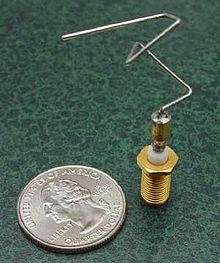
\includegraphics[height=100px]{elias/images/antenna.jpg}
    \caption{\url{en.wikipedia.org/wiki/genetic_algorithm}}
  \end{figure}
\end{frame}

\subsection{Structuring Candidate Solutions}

\begin{frame}{Genetic Algorithms using Neural Networks}
  picture of use of neural networks

  bit strings as chromosomes to be manipulated
\end{frame}

\section{Existing methods}

\begin{frame}{Hamming distance}
  illustration of the workings of hamming distance
\end{frame}

\begin{frame}{Fitness-based}
  illustration of the workings of fitness-based
\end{frame}

\begin{frame}{What do they miss?}
  weaknesses and such
\end{frame}

